\documentclass{beamer}
\usetheme{CambridgeUS}
\title[Process]{The Koopman operator identification algorithm}
\subtitle{So far}
\institute[Polimi]{Politecnico di Milano}
\author{Sergio Vanegas}
\date{\today}

\usepackage{listings}
\usepackage[framed,numbered,autolinebreaks,useliterate]{mcode/mcode}

\usepackage{xcolor}

\usepackage{siunitx}

\usepackage{caption}
\usepackage{subcaption}

\begin{document}

\begin{frame}[plain,noframenumbering]
    \maketitle
\end{frame}

\begin{frame}{Table of Contents}
    \tableofcontents
\end{frame}


\section{Robust Koopman}

\begin{frame}{Frobenius regularization - Formulation}
    We start by following the proposed reformulation of the minimization problem proposed in \textit{Robust tube-based model predictive control with Koopman operators} as follows:

    \begin{equation*}
        \overline{\mathcal{K}}_N =
        \min_{\mathcal{K} \in \mathbb{R}^{\tilde{N} \times N}}
        \sum_{k=1}^K \left[
            \left|\left|
                \mathbf{g}\left(\mathbf{y}\left[k\right]\right) - 
                \mathcal{K}
                \begin{pmatrix}
                \mathbf{g}\left(\mathbf{x}\left[k\right]\right)
                \\
                \mathbf{u}\left[k\right]
                \end{pmatrix}
            \right|\right|^2
            {
                \color{red}
                + \alpha\left|\left|\mathcal{K}\right|\right|_F^2
            }
        \right],
    \end{equation*}

    where

    \begin{itemize}
        \item $\mathbf{g}$ is the observable vector,
        \item $K$ is the total number of snapshots,
        \item $\left(\mathbf{x},\mathbf{y}\right)$ are the snapshot pairs,
        \item $\mathbf{u}$ is the input vector,
        \item $\left|\left|\cdot\right|\right|_F$ is the element-wise 2-norm (Frobenius norm).
    \end{itemize}
\end{frame}

\begin{frame}[fragile]{Frobenius regularization - MATLAB implementation}
    In order to properly minimize the regularized formulation, an external Toolbox that exploited its convexity had to be integrated. In our case, CVX was used.

    \begin{lstlisting}[language=Matlab,basicstyle=\tiny]
function [A,B] = Koopman(X,Y,U,alpha)
    % Following "Practical Considerations" from Korda-Mezic + Williams

    A = zeros(size(Y,1),size(X,1));
    B = zeros(size(Y,1),size(U,1));

    for i=1:size(Y,1)
        % In the real implementation, a skip is called when alpha=0
        cvx_begin
            variable m(length)
            minimize (norm(m*[X;U]-Y(i,:)) + alpha*norm(m))
        cvx_end

        A(i,:) = m(1:size(X,1));
        B(i,:) = m(size(X,1)+1:end);
    end
end
    \end{lstlisting}
\end{frame}

\begin{frame}{Frobenius regularization - Results I}
    The regularization technique was put to the test with both a \textit{clean} and a \textit{noisy} dataset, using a clean simulation as reference during the benchmarks.

    \begin{figure}
        \centering
        \begin{subfigure}[b]{0.45\textwidth}
            \centering
            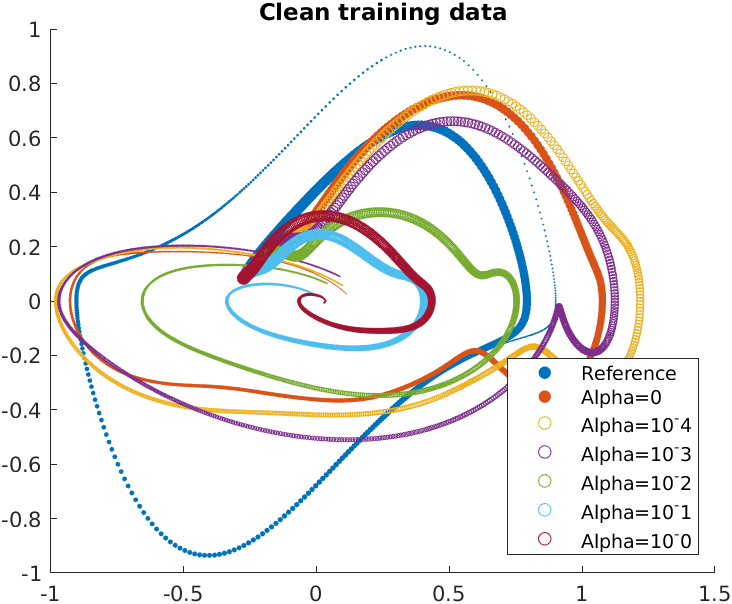
\includegraphics[width=\textwidth]{Clean_Training.png}
            \caption{Clean training dataset}
            \label{fig:Koopman_clean}
        \end{subfigure}
        \hfill
        \begin{subfigure}[b]{0.45\textwidth}
            \centering
            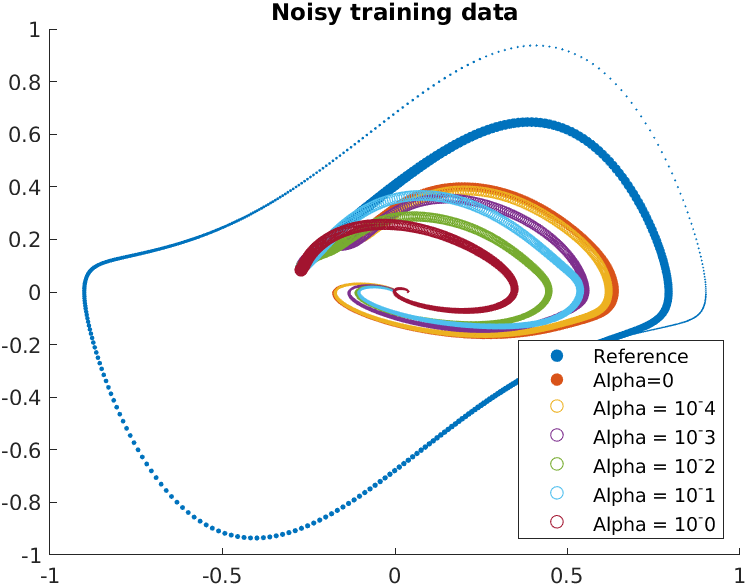
\includegraphics[width=\textwidth]{Noisy_Training.png}
            \caption{Noisy training dataset}
            \label{fig:Koopman_noisy}
        \end{subfigure}
        \caption{Frobenius regularized Koopman operator}
        \label{fig:Koopman_Frobenius}
    \end{figure}
\end{frame}

\begin{frame}{Frobenius regularization - Results II}
    \begin{figure}
        \centering
        \begin{subfigure}[b]{0.45\textwidth}
            \centering
            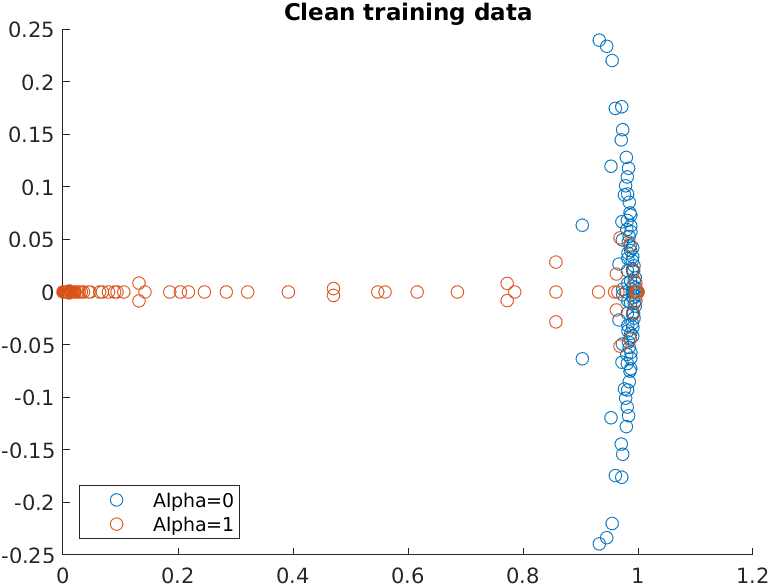
\includegraphics[width=\textwidth]{Clean_Eigen.png}
            \caption{Clean training dataset}
            \label{fig:Eigen_clean}
        \end{subfigure}
        \hfill
        \begin{subfigure}[b]{0.45\textwidth}
            \centering
            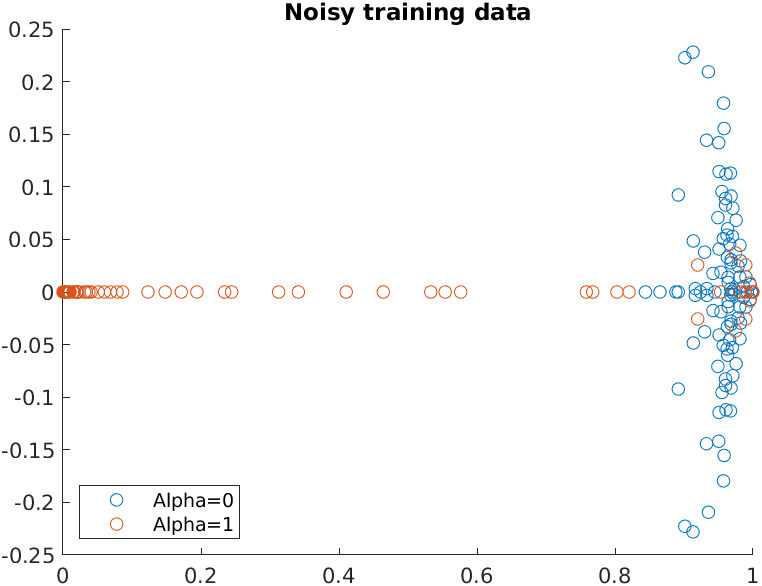
\includegraphics[width=\textwidth]{Noisy_Eigen.png}
            \caption{Noisy training dataset}
            \label{fig:Eigen_noisy}
        \end{subfigure}
        \caption{Frobenius regularized eigenvalues}
        \label{fig:Eigen_Frobenius}
    \end{figure}
\end{frame}


\section{From prototyping to implementation}

\begin{frame}{Language alternatives - Benchmark formulation}
    Considering the performance limitations of a high-level interpreted languages, some alternatives had to be considered. The evaluated candidates were:

    \begin{itemize}
        \item Python: still high-level, but further optimized because of its open-source nature. Both an open-source clone of CVX (cvxpy) and a mat file utility are included in the scipy official package.
        \item C++: compiled language, and a classical choice for scientific programming. Even if complex, the development process is facilitated by the availability of the CPLEX API.
        \item Rust: memory-safe compiled language that pretends to replace C/C++ in the following years. High development complexity given it's in its early stages.
    \end{itemize}

    A simple benchmark based on the performance of ODE data generation (which evaluates both matrix and nonlinear implementations) was set up.
\end{frame}

\begin{frame}{Language alternatives - Benchmark results}

    \begin{itemize}
        \item MATLAB

        \begin{itemize}
            \item User time: $\SI{26.05}{\second}$
            \item Wall clock time: $\SI{28.62}{\second}$
            \item Maximum resident set size: $782348$ kb
        \end{itemize}

        \item Python

        \begin{itemize}
            \item User time: $\SI{25.44}{\second}$
            \item Wall clock time: $\SI{26.21}{\second}$
            \item Maximum resident set size: $59880$ kb
        \end{itemize}

        \item C++
        
        \begin{itemize}
            \item User time: $\SI{0.70}{\second}$
            \item Wall clock time: $\SI{1.76}{\second}$
            \item Maximum resident set size: $4320$ kb
        \end{itemize}

        \item Rust
        
        \begin{itemize}
            \item User time: $\SI{0.54}{\second}$
            \item Wall clock time: $\SI{6.44}{\second}$
            \item Maximum resident set size: $2736$ kb
        \end{itemize}
    \end{itemize}
    
\end{frame}

\begin{frame}{Language alternatives - Accuracy verification}
    \begin{figure}
        \centering
        \begin{subfigure}[b]{0.3\textwidth}
            \centering
            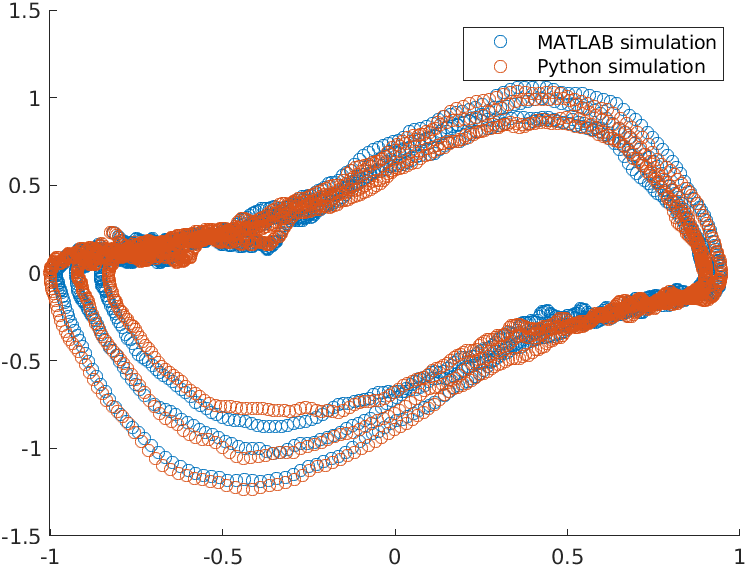
\includegraphics[width=\textwidth]{Python_Sim.png}
            \caption{Python - Simulated trajectory}
            \label{fig:sim_python}
        \end{subfigure}
        \hfill
        \begin{subfigure}[b]{0.3\textwidth}
            \centering
            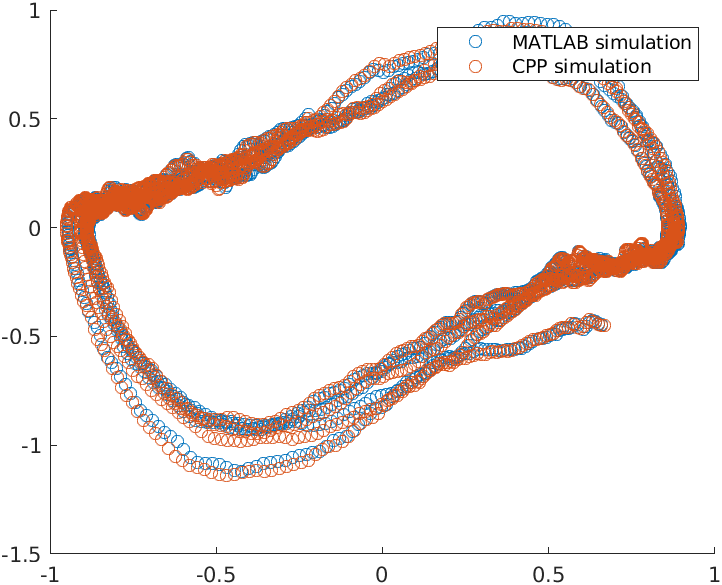
\includegraphics[width=\textwidth]{Cpp_Sim.png}
            \caption{C++ - Simulated trajectory}
            \label{fig:sim_cpp}
        \end{subfigure}
        \hfill
        \begin{subfigure}[b]{0.3\textwidth}
            \centering
            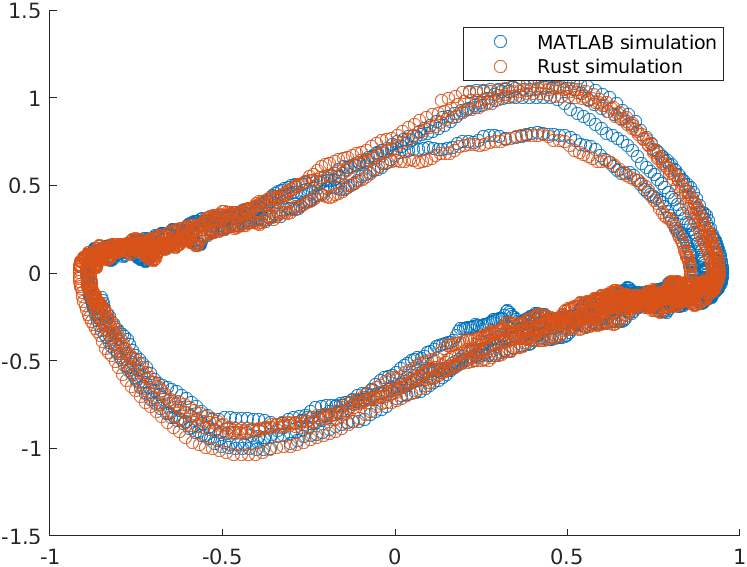
\includegraphics[width=\textwidth]{Rust_Sim.png}
            \caption{Rust - Simulated trajectory}
            \label{fig:sim_rust}
        \end{subfigure}
        \caption{Simulated trajectories (MATLAB simulation as reference)}
        \label{fig:implementations}
    \end{figure}
\end{frame}


\section{Extended Dynamic Mode Decomposition}

\begin{frame}{EDMD - Theory I}
    We derive the procedure from Williams et Al.: having calculated the Koopman matrix projection, we find the Koopman eigenvalue/eigenvector pairs for the $A$ matrix s.t.

    \begin{equation*}
        A^T \mathbf{\xi}_j = \mu_j \mathbf{\xi}_j \quad , \quad j \in \left\{1,\dots,\tilde{N}\right\}
    \end{equation*}

    The reason why we find the eigenvectors of the transposed is because each row of the $A$ matrix is associated to a single observable, but in the Eigen procedure we need the opposite.
    
    Having obtained all the aforementioned pairs, we define an eigenfunction as the projection of an observable vector over each eigenvector, just as follows

    \begin{equation*}
        \phi_j\left(\mathbf{x}\right) = \mathbf{g}\left(\mathbf{x}\right)^T \mathbf{\xi}_j
    \end{equation*}
\end{frame}

\begin{frame}{EDMD - Theory II}
    Exploiting the linearity of the operator and the Eigenvalue theory, we express the Koopman operator as follows:
    
    \begin{align*}
        \mathbf(\phi_j)\left(\mathbf{y}\right)
        &=
        \mathbf{g}\left(\mathbf{y}\right)^T \mathbf{\xi}_j \\
        &=
        \left(\overline{\mathcal{K}}_N
        \begin{pmatrix}
            \mathbf{g}\left(\mathbf{x}\right)
            \\
            \mathbf{u}
        \end{pmatrix}\right)^T \mathbf{\xi}_j \\
        &=
        \begin{pmatrix}
            \mathbf{g}\left(\mathbf{x}\right)^T
            &
            \mathbf{u}^T
        \end{pmatrix}
        \left(
            \begin{pmatrix}
                A^T
                \\
                B^T
            \end{pmatrix}
            \mathbf{\xi}_j
        \right) \\
        &=
        \mu_j \phi_j\left(\mathbf{x}\right)
        +
        \mathbf{u}^T B^T \mathbf{\xi}_j \\
        &=
        \mu_j \phi_j\left(\mathbf{x}\right)
        +
        \mathbf{\xi}_j^T B \mathbf{u}
    \end{align*}

    The last equivalence is possible because, at that point, we are dealing with a scalar value. 
\end{frame}

\begin{frame}{EDMD - Theory III}
    From this form, we can derive the full eigenspace decomposition by concatenating the $\phi$-projections vertically as follows

    \begin{equation*}
        \Phi\left(\mathbf{y}\right) = M \Phi\left(\mathbf{x}\right) + \Xi^T B \mathbf{u}
    \end{equation*}

    where $M$ is a diagonal matrix containing the eigenvalues ordered w.r.t. the horizontal concatenation of the vertical vectors $\xi_j$ in $\Xi$.

    At this point, it is easy to see that the original observables are recoverable at any point through the expression

    \begin{align*}
        \Phi\left(\mathbf{x}\right)^T &= \mathbf{g}\left(\mathbf{x}\right)^T \Xi \\
        \implies \left[\Xi^T\right]^{-1} \Phi\left(\mathbf{x}\right) &= \mathbf{g}\left(\mathbf{x}\right)
    \end{align*}
\end{frame}

\begin{frame}[fragile]{Implementation - Eigenpair extraction and discrimination}
    We start by extracting the eigenpairs with the following line: \mcode{[~,Mu,Xi] = eig(A);}. For numerical reasons, we request the left eigenvectors of the original matrix instead of the right eigenvectors of the transposed matrix.

    Then, we discriminate irrelevant eigenvectors by setting a magnitude threshold as follows:

    \begin{lstlisting}[language=Matlab]
thr = 0.1;
idx_r = abs(diag(Mu))>thr;
Xi_r = Xi(:,idx_r);
Mu_r = Mu(idx_r,idx_r);
    \end{lstlisting}    
\end{frame}

\begin{frame}[fragile]{Implementation - Projection tracking and observable reconstruction}
    Finally, we track the trajectory exclusively in the eigenspace with the filtered pairs, and then reconstruct the original observables (and from those, the states) as follows:

    \begin{lstlisting}[language=Matlab]
Phi = zeros(length(Mu_r),L);
Phi(:,1) = Xi_r'*g_p(:,1);

for i=1:L-1
    Phi(:,i+1) = Mu_r*Phi(:,i) + Xi_r'*B*u(:,i);
end

g_eig = Xi_r'\Phi;
z_eig = C*g_eig;
    \end{lstlisting}
\end{frame}

\begin{frame}{EDMD decomposition - Results}
    \begin{figure}
        \centering
        \begin{subfigure}[b]{0.3\textwidth}
            \centering
            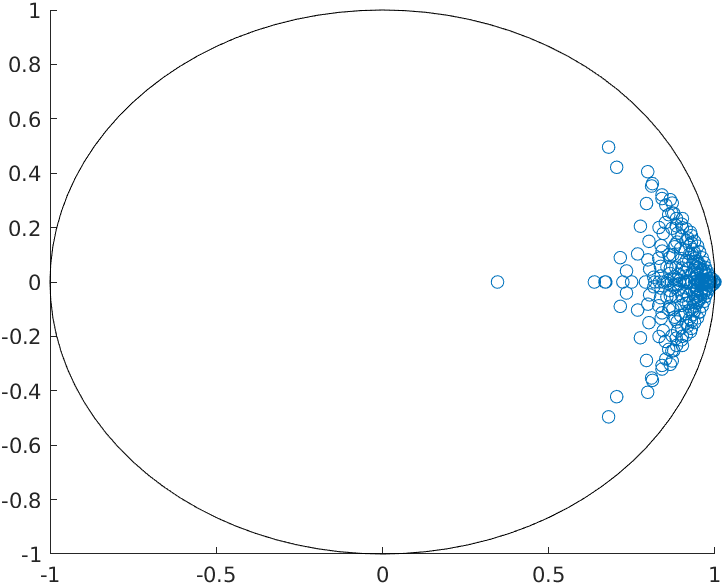
\includegraphics[width=\textwidth]{EDMD_Ref.png}
            \caption{Eigenvalues - M=300}
            \label{fig:EDMD_Ref}
        \end{subfigure}
        \begin{subfigure}[b]{0.3\textwidth}
            \centering
            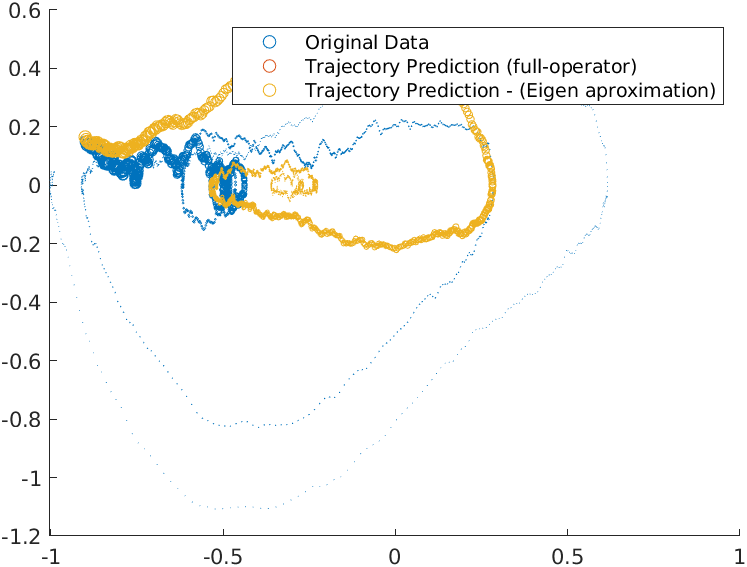
\includegraphics[width=\textwidth]{EDMD_00.png}
            \caption{EDMD - Unfiltered}
            \label{fig:EDMD_00}
        \end{subfigure}
        \\
        \begin{subfigure}[b]{0.3\textwidth}
            \centering
            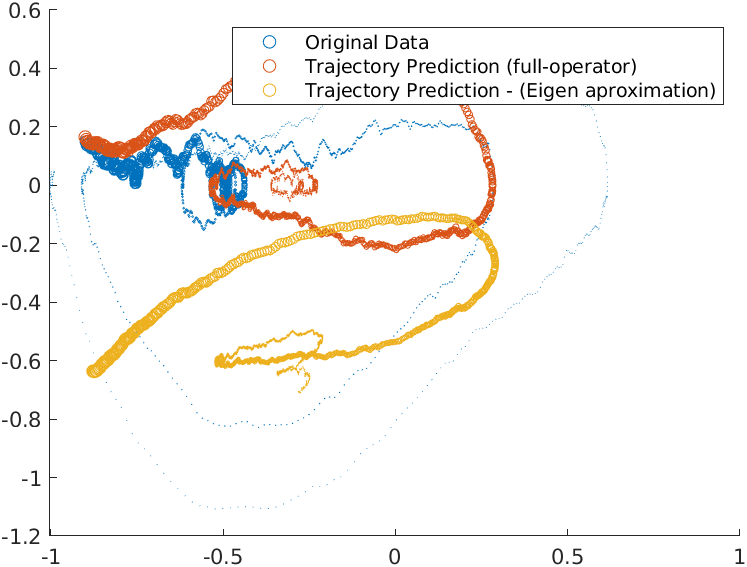
\includegraphics[width=\textwidth]{EDMD_50.png}
            \caption{EDMD - Thr = 0.5}
            \label{fig:EDMD_50}
        \end{subfigure}
        \begin{subfigure}[b]{0.3\textwidth}
            \centering
            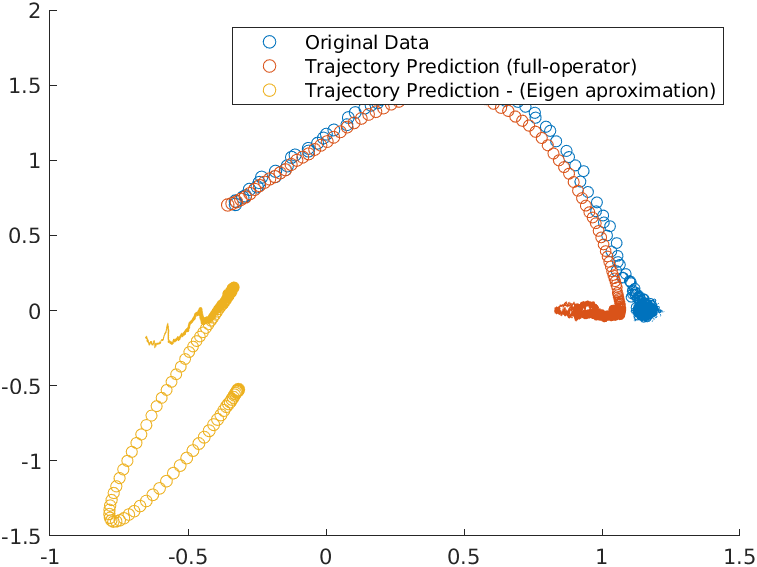
\includegraphics[width=\textwidth]{EDMD_70.png}
            \caption{EDMD - Thr = 0.70}
            \label{fig:EDMD_70}
        \end{subfigure}
        \label{fig:EDMD}
   \end{figure}
\end{frame}


\section{Conclusions}

\begin{frame}[allowframebreaks]{Conclusions}
    \begin{itemize}
        \item The Frobenius regularization does not visibly blind the identification algorithm from relatively low measurement noise; nevertheless, it does make it more resistant to instabilities, which we can easily verify by observing the eigenvalues moving towards the origin when increasing the value of $\alpha$.
        \item For larger datasets/higher dimension systems, MATLAB is no longer a viable framework to calculate the matrix approximation of the Koopman operator. C++ stands as the preferred language given its standardization and low memory consumption; Python, however, already improves significantly the memory efficiency on its own (even though the execution time does not change to a measurable degree).
        \item Nevertheless, both MPC and eigenvalue decomposition can be applied to the operator in MATLAB once the projection has been calculated through a lower-level implementation. The data management method now has to be switched from a proprietary \textit{mat file} approach to a cross-compatible \textit{csv} approach.
        \item EDMD does present an opportunity to reduce computational load in real scenarios, since eigenvectors associated to numerically insignificant eigenvectors produced by measurement noise can be removed when handling a high-dimensional observable/state space. Integration with the regularized method should provide a solid identification framework, although a more realistic scenario is required in order to verify that hypothesis.
    \end{itemize}
\end{frame}

\end{document}